

\documentclass[11pt]{article}
\usepackage{graphicx}
\usepackage[margin=1.25in]{geometry}
\usepackage[usenames,dvipsnames]{color}
\usepackage{url}
\usepackage[colorlinks = true,
            linkcolor = blue,
            urlcolor  = blue,
            citecolor = blue,
            anchorcolor = blue]{hyperref}
%can change bib here...
\usepackage[square,comma,sort&compress,numbers]{natbib}
\bibliographystyle{unsrtnat}


%%%%%%%%%%%%%%%%%%%%%%%%%%%%%%%%%%%%%%%%%%%%%%%%%%%%%%%%%%%%%%%%%%%%
% basic data for the eprint:
%%%%%%%%%%%%%%%%%%%%%%%%%%%%%%%%%%%%%%%%%%%%%%%%%%%%%%%%%%%%%%%%%%%%

\textwidth=6.0in  \textheight=8.5in

%%  Adjust these for your printer:
\parskip=0.1truein 
  
%% preprint number data:
\newcommand\pubnumber{Preprint Number Goes Here?}
\newcommand\pubdate{\today}



%%%%%%%%%%%%%%%%%%%%%%%%%%%%%%%%%%%%%%%%%%%%%%%%%%%%%%%%%%%%%%%%%%%%%%%%%%%%
%   document style macros
%%%%%%%%%%%%%%%%%%%%%%%%%%%%%%%%%%%%%%%%%%%%%%%%%%%%%%%%%%%%%%%%%%%%%%%%%%%%
\def\Title#1{\begin{center} {\LARGE #1 } \end{center}}
\def\Author#1{\begin{center}{ \sc #1} \end{center}}
\def\Address#1{\begin{center}{ \it #1} \end{center}}
\def\andauth{\begin{center}{and} \end{center}}
\def\submit#1{\begin{center}Submitted to {\sl #1} \end{center}}
\newcommand\pubblock{\rightline{\begin{tabular}{l} \pubnumber\\
         \pubdate \end{tabular}}}
\newenvironment{Abstract}{\begin{quotation} \begin{center}
                       ABSTRACT
     \end{center}\bigskip  }{\end{quotation}}
\newenvironment{Presented}{\begin{quotation} \begin{center} 
             CONTRIBUTED TO\end{center}\bigskip 
      \begin{center}\begin{large}}{\end{large}\end{center} \end{quotation}}
\def\submit#1{\begin{center}Submitted to {\sl #1} \end{center}}
\def\Acknowledgements{\bigskip  \bigskip \begin{center} \begin{large}
             \bf ACKNOWLEDGEMENTS \end{large}\end{center}}
%%%%%%%%%%%%%%%%%%%%%%%%%%%%%%%%%%%%%%%%%%%%%%%%%%%%%%%%%%%%%%%%%%%%%%%%%%%%
%  personal abbreviations and macros

\input workshopsymbols.tex

\newcommand\snowmass{\begin{center}\rule[-0.2in]{\hsize}{0.01in}\\\rule{\hsize}{0.01in}\\
\vskip 0.1in Submitted to the  Proceedings of the US Community Study\\ 
on the Future of Particle Physics (Snowmass 2021)\\ 
\rule{\hsize}{0.01in}\\\rule[+0.2in]{\hsize}{0.01in} \end{center}}

%%%%%%%%%%%%%%%%%%%%%%%%%%%%%%%%%%%%%%%%%%%%%%%%%%%%%%%%%%%%%%%%%%%%%%%%%%%

\begin{document}

\pubblock

\Title{Summarizing experimental sensitivities of collider experiments to Dark Matter models and comparison to other experiments}

\bigskip 

\Author{Add Your Name Here}

%LOI authors:
%\noindent{\large \bf Authors: }Antonio Boveia (Ohio State University), Linda Carpenter (Ohio State University), Caterina Doglioni (Lund University), William Kalderon (Brookhaven National Lab), Boyu Gao (Ohio State University), Philip Coleman Harris (Massachusetts Institute of Technology), David Yu (Brown University)\\

%\medskip

%\Address{ c/o  R. W. Emerson, Concord, MA USA}

\medskip

 \begin{Abstract}
\noindent Plots summarizing the constraints on Dark Matter (DM) models can help visualize synergies between different searches for the same kind of experiment, as well as between different experiments. 
In this LOI, we propose to produce these plots from the perspective of collider searches within EF10 starting from inputs from future collider facilities. We will take as a starting point the plots currently made for LHC searches and recommended by the Dark Matter Working Group, also used for the BSM and Dark Matter chapters of the European Strategy Briefing Book. We also intend to actively participate in the cross-frontier discussions about dark matter complementarity. 
\end{Abstract}


\snowmass

\def\thefootnote{\fnsymbol{footnote}}
\setcounter{footnote}{0}
%

\section{Introduction}

Astrophysical and cosmological evidence has indicated the existence of Dark Matter (DM). Among the particle physics experiments probing DM, collider experiments aim to detect the production of invisible DM particles as well as the visible decay of the particle(s) mediating such a process~\cite{Kahlhoefer:2017dnp}. This approach sets model-dependent constraints complementary to other types of DM experiments, including indirect detections (ID) of DM annihilation at sky and direct detections (DD) of DM-nucleon scattering in terrestrial detectors.

\section{Plots summarizing collider reach to dark matter mediator models}

\subsection{Previous text from LOI}

To compare how existing collider searches may discover or constrain a given model, and to understand how future collider experiments would extend these results, we propose to make summary plots like Figure\ref{fig:Fig1} ~\cite{CMSSummary,ATL-PHYS-DMSUM-JHEP-2019} in terms of the fundamental parameters of the Lagrangian of a model. 
Exclusion comparisons in the DM mass – mediator mass plane (left panel) combine searches for both invisible and visible signals of the model. Summary plots such as on the mediator – quark coupling and mediator mass plane (right panel) target the production coupling and visible decay of the mediator. For both types of plots, we suggest using DM simplified models~\cite{ABERCROMBIE2020100371} since they are simple descriptions of collider phenomenology that capture common features across many full models, while ignoring the differences among these models at energies higher than collider scales~\cite{doi:10.1146/annurev-nucl-101917-021008}. In the simplified models, the interaction between Standard Model (SM) particles and DM is mediated by a new particle called a mediator, where the mediator – quark coupling controls the interaction strength between mediator and SM quarks. These models can also be used as a stepping stone to connect collider searches to accelerator searches since these results can be reinterpreted using different portal models~\cite{Beacham:2652223}, as the simplified models we are using are very close to other portal models. 

\begin{figure}[ht]
\begin{tabular}{ll}
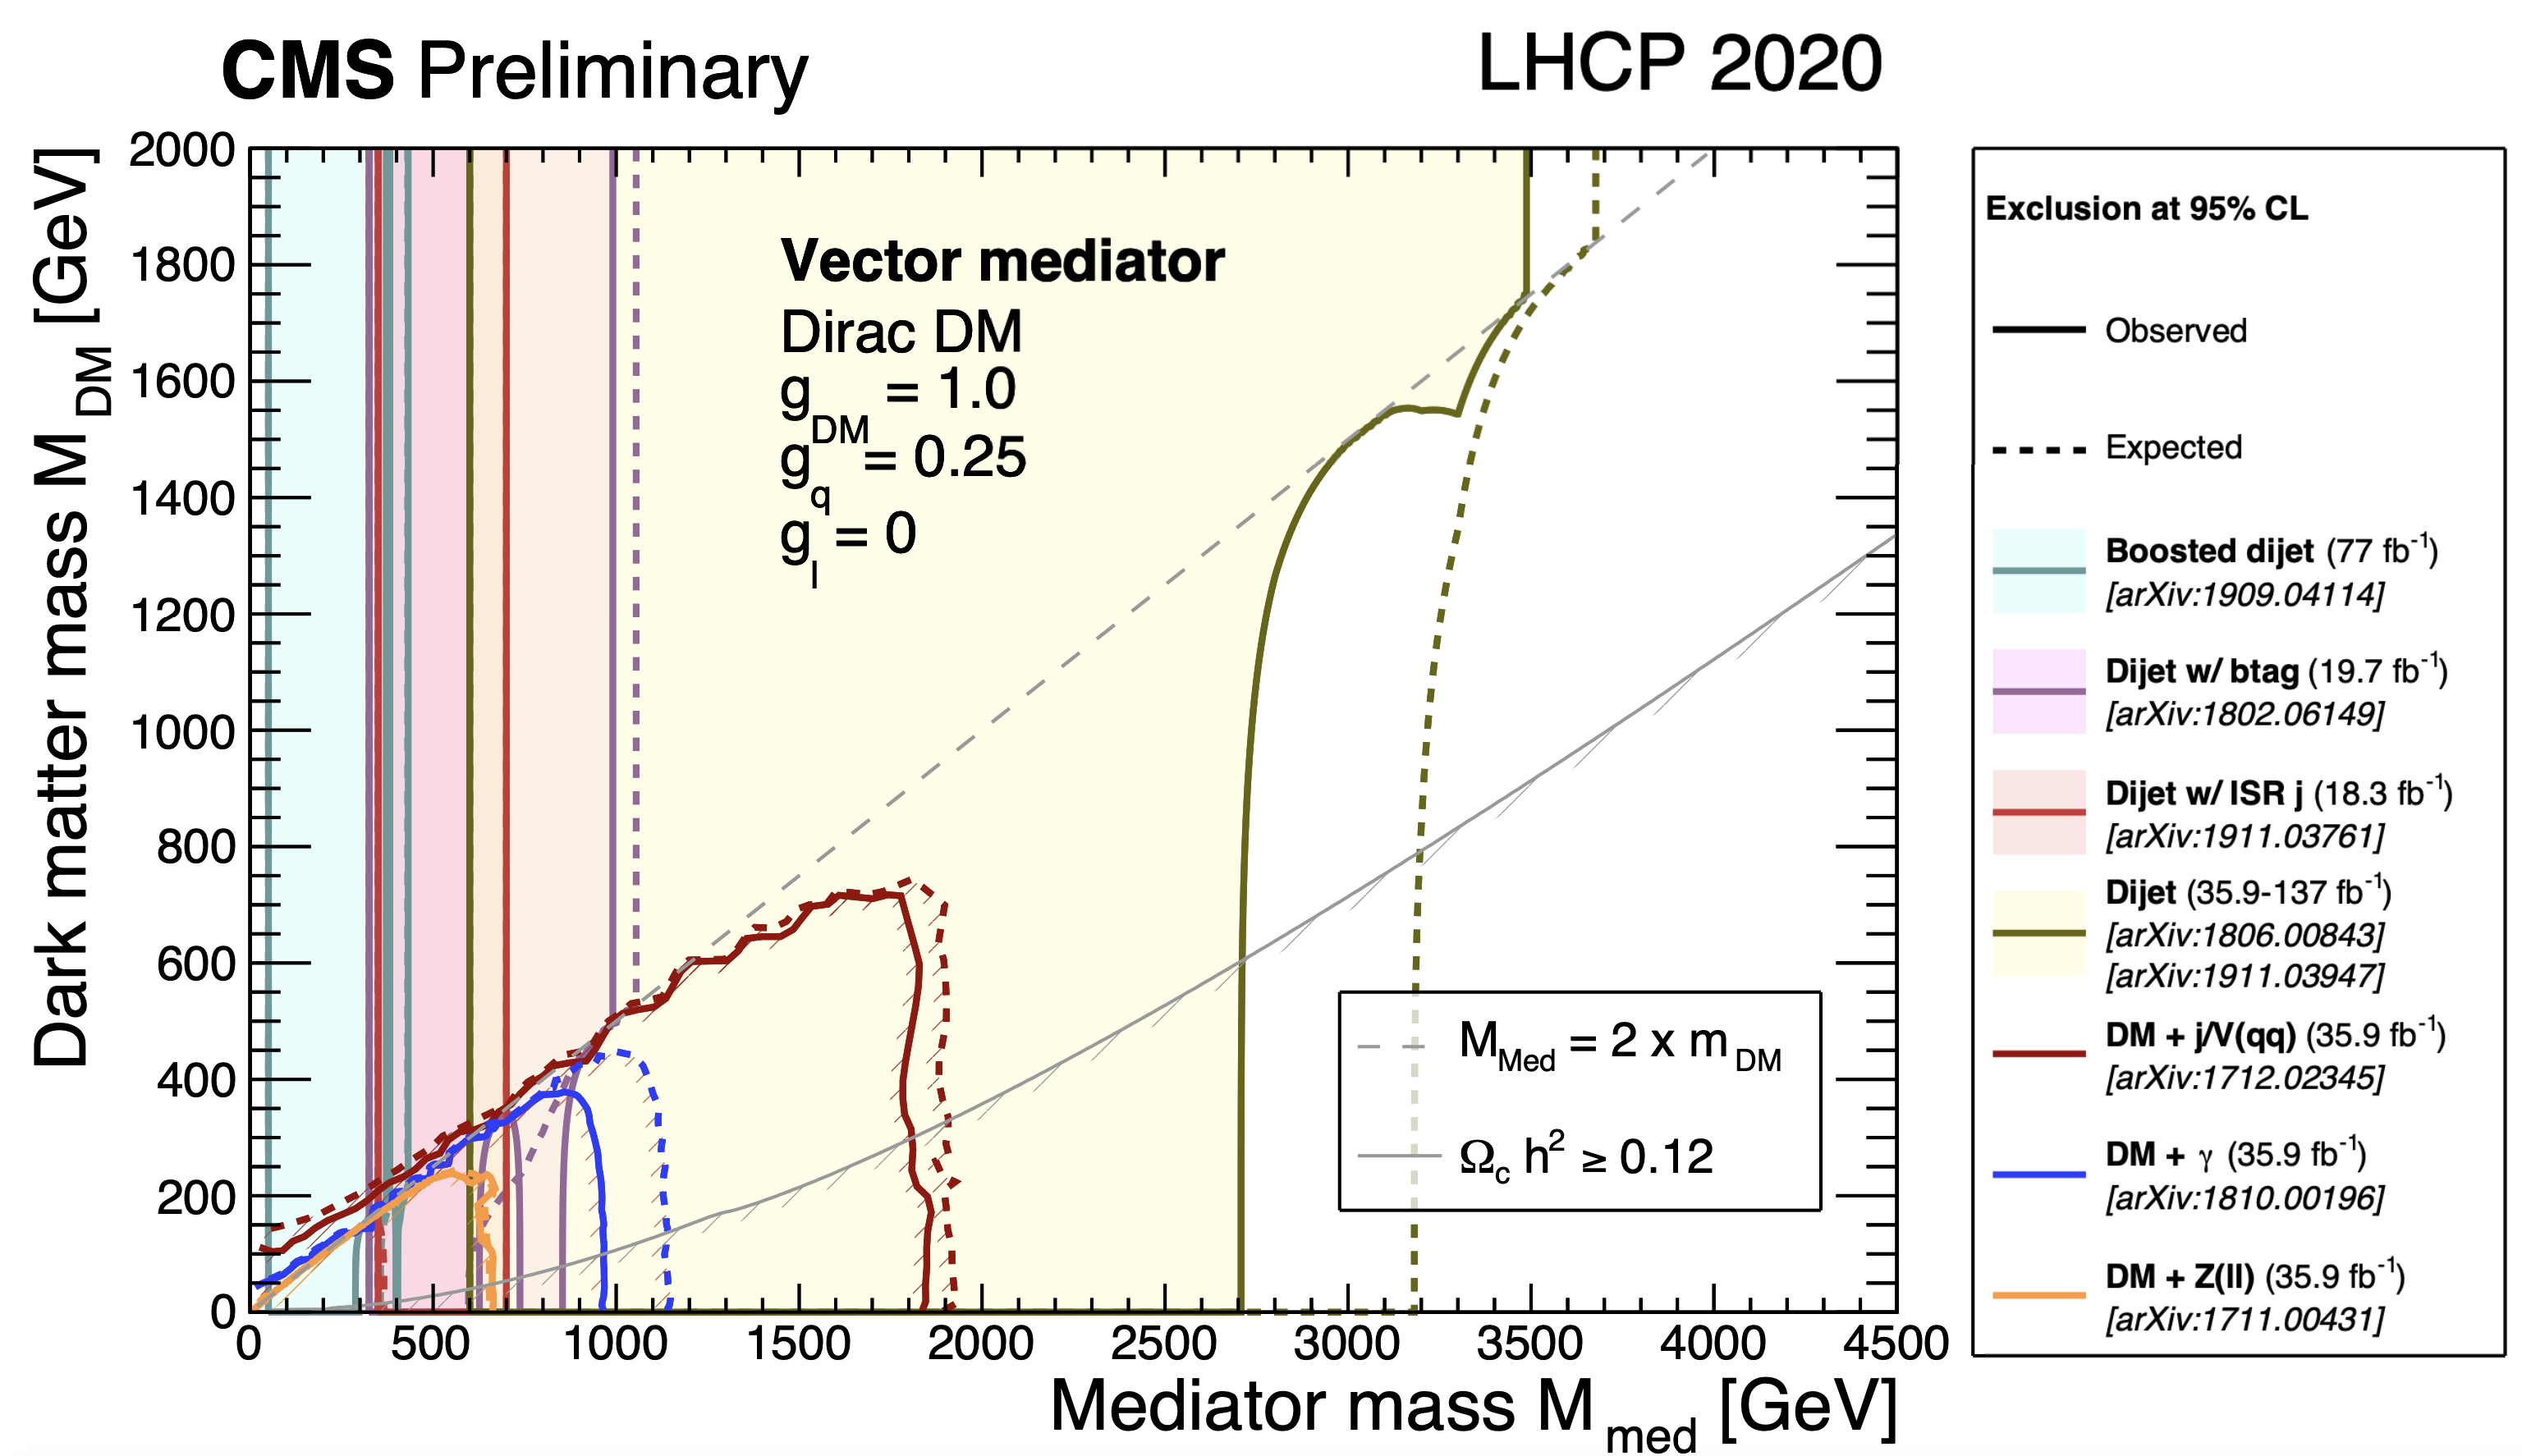
\includegraphics[scale=0.17]{DMsummaryplots_med_dm.png}
&
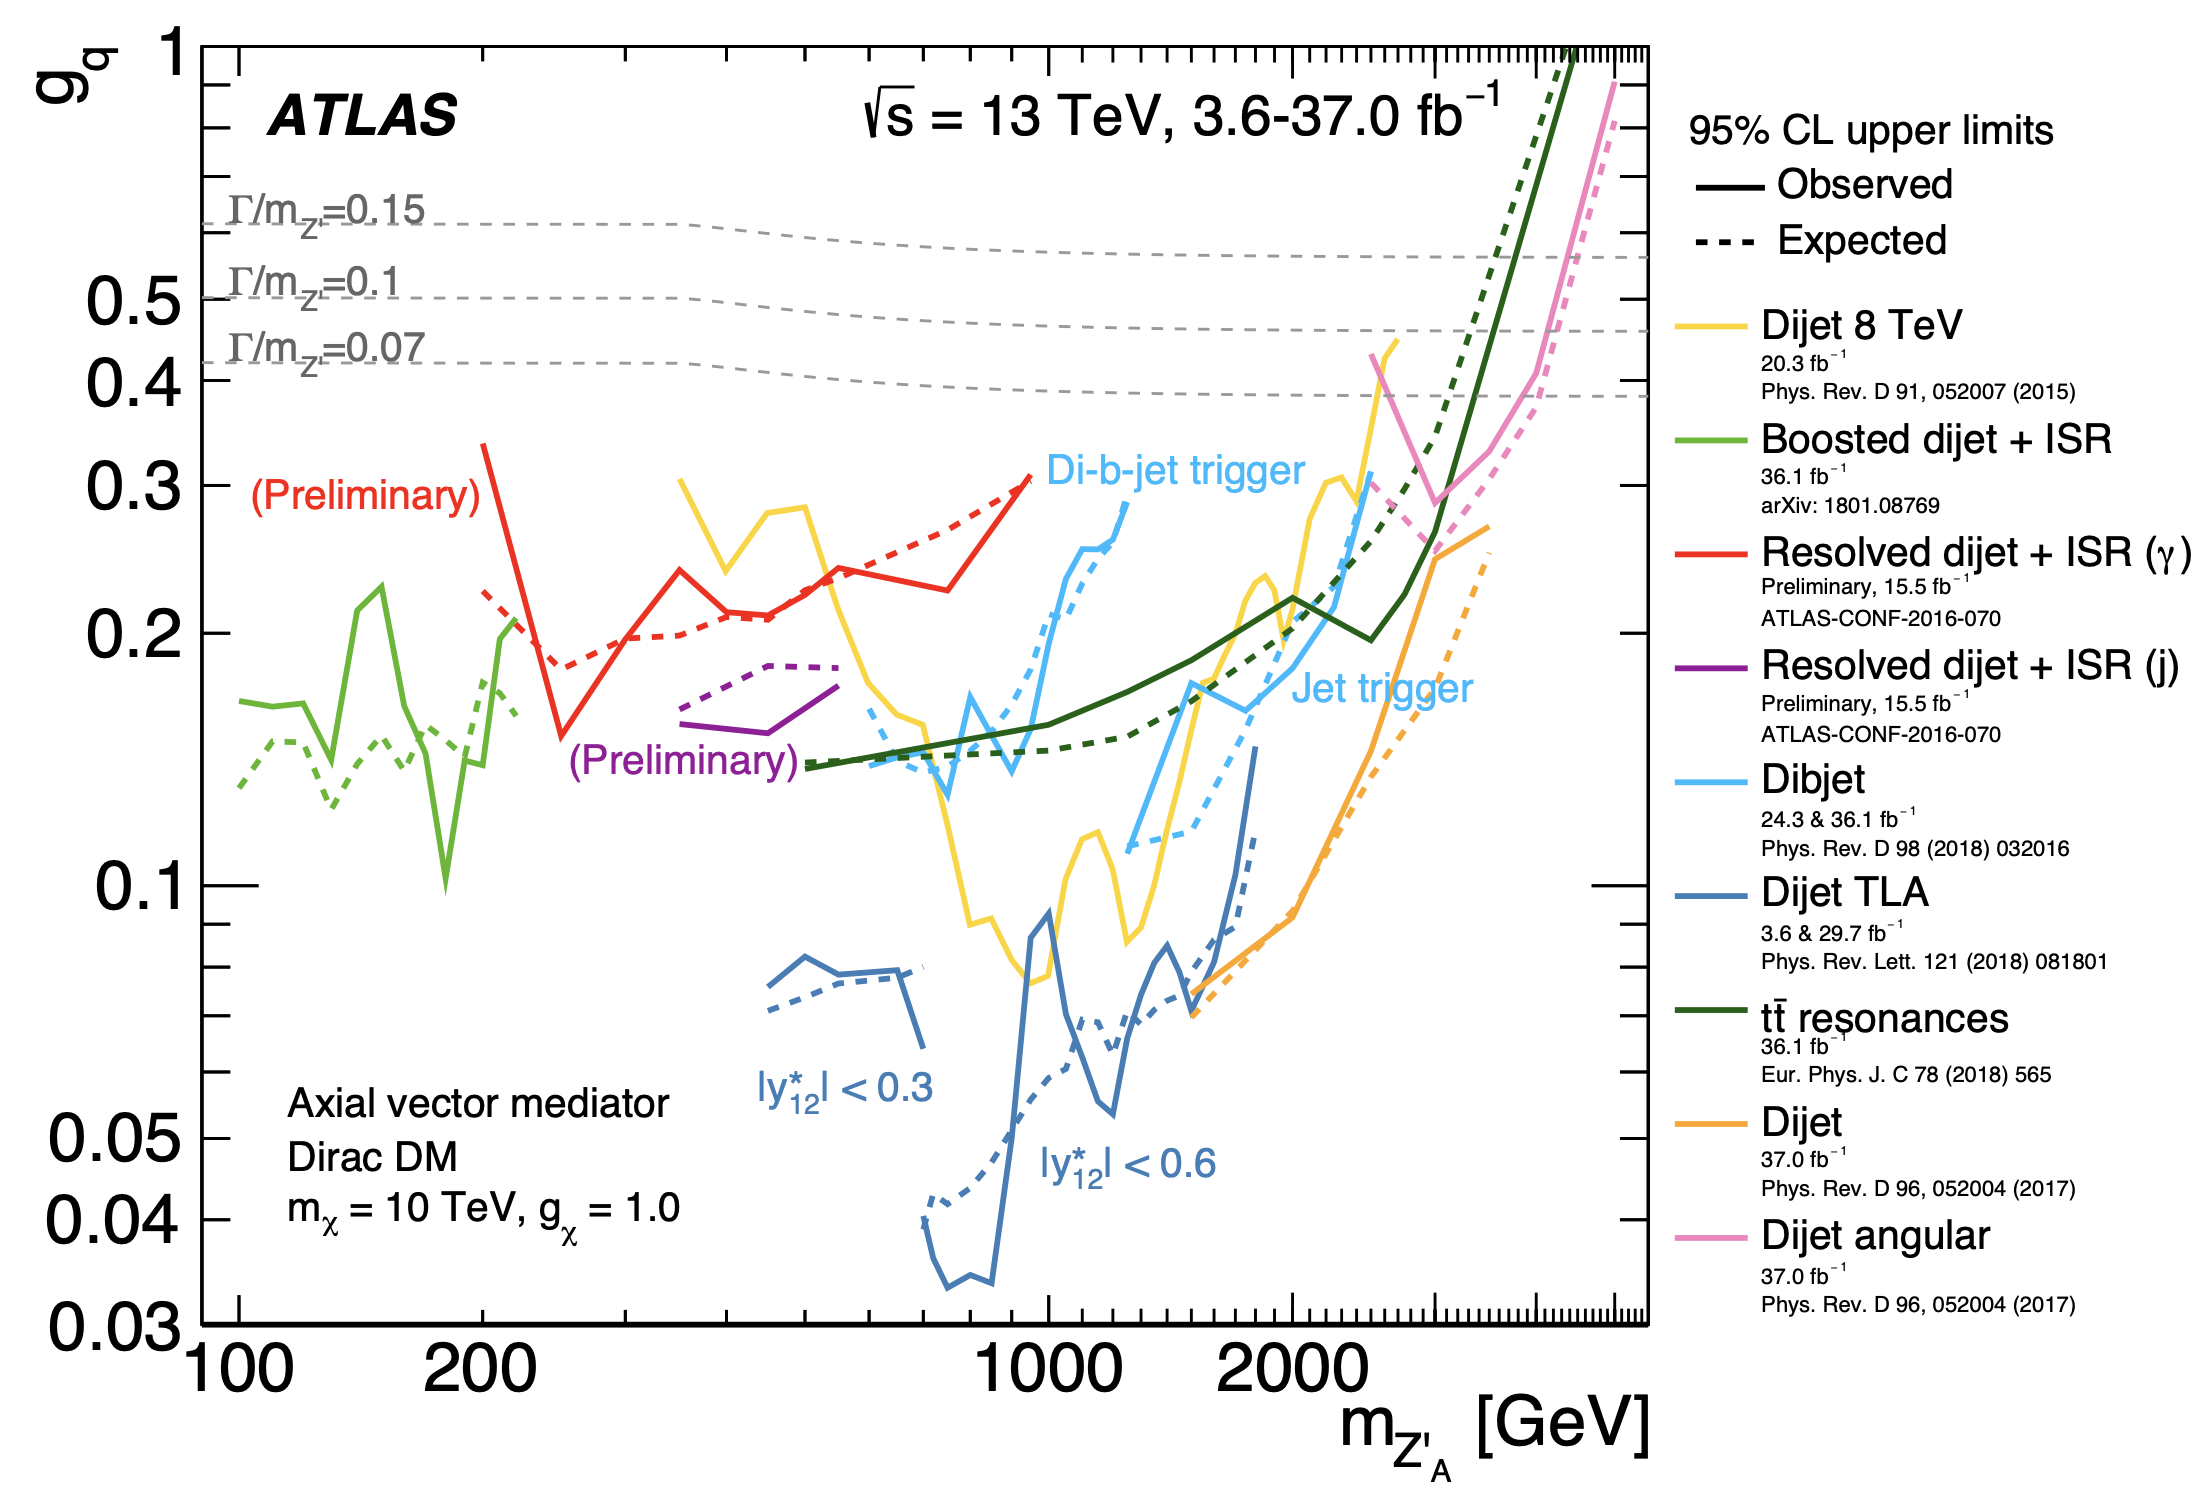
\includegraphics[scale=0.185]{DMsummaryplots_med_gq.png}
\end{tabular}
\caption{{\bf Left panel}: regions in DM mass - mediator mass plane excluded at 95$\%$ CL by visible and invisible searches for DM vector simplified models. {\bf Right panel}: Dijet search contours for 95$\%$ CL upper limits on the coupling $g_{q}$ as a function of resonance mass $m_{Z'_{A}}$ for axial-vector simplified models. The expected limits from each search are indicated by dotted lines. Left panel adapted from CMS Dark Matter summary plots~\cite{CMSSummary}, right panel adapted from ATLAS Dark Matter summary plots~\cite{ATL-PHYS-DMSUM-JHEP-2019}.
}
\label{Fig:Fig1}
\end{figure}

\subsection{Models considered}

\subsection{Results}

\section{Comparisons to other experiments}

\subsection{Previous text from LOI}

To understand how present and future collider searches complement present and future ID and DD experiments, we also propose to compare collider searches together with other experiments using variables commonly employed by displaying indirect and direct detection results, using the methods recommended by the LHC Dark Matter Working Group (DM WG)~\cite{BOVEIA2020100365,ALBERT2019100377}. An example of such plots (using fixed mediator – quark couplings) is shown in Figure \ref{Fig:Fig2}~\cite{Ellis:2691414}. Here, we propose to use results from work undergoing in synergy between the LHC DM WG and the Snowmass community~\cite{LOIVaryingCouplings} on collider limits with lower mediator - quark coupling values, rather than only for the fixed coupling values proposed by the LHC DM WG ~\cite{BOVEIA2020100365,ALBERT2019100377} and used in the European Strategy Briefing Book~\cite{Ellis:2691414}. This work will allow us to have a more complete picture of the complementarity of collider DM searches with direct and indirect detection, as well as compare collider results with collaborations that are sensitive to much lower couplings, such as accelerator-based and fixed target experiments. 

We are particularly interested in how to improve these plots in cooperation with the DD, ID and astrophysics probes communities within the Cosmic Frontier (CF1, CF3) and to contribute to summary plots where DM collider results and projections are shown together with those of accelerator-based experiments within the Rare and Precision Frontier (RF6). 

\begin{figure}[ht]
\begin{tabular}{ll}
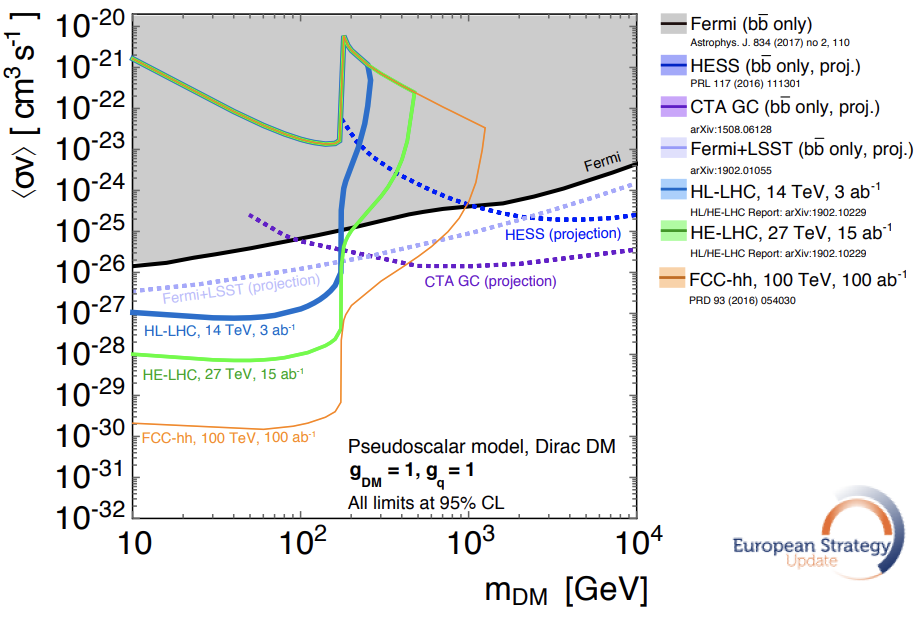
\includegraphics[scale=0.52]{DMsummaryplots_ID.png}
&
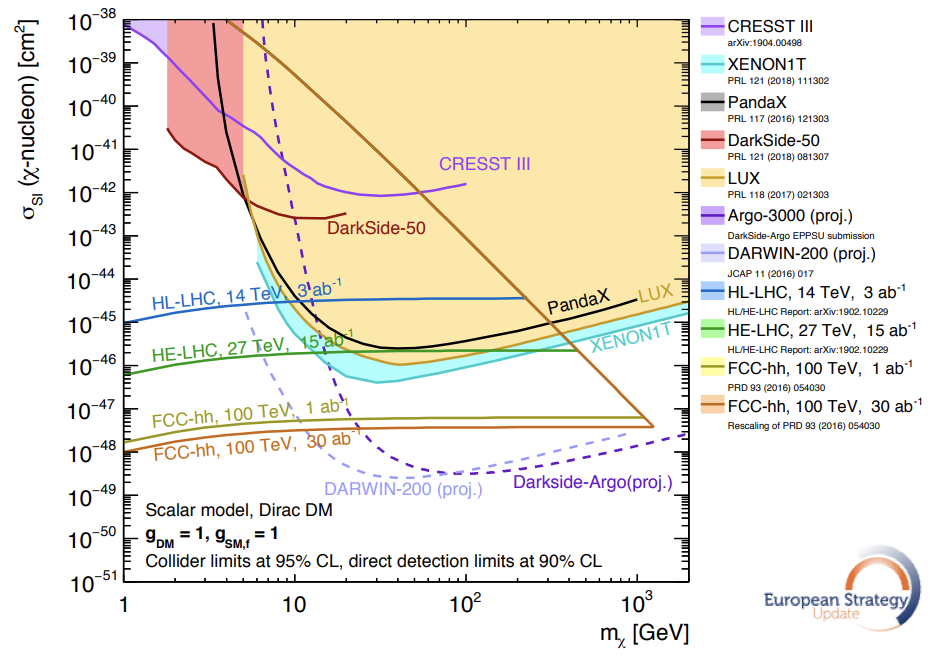
\includegraphics[scale=0.49]{DMsummaryplots_DD.png}
\end{tabular}
\caption{{\bf Left panel}: comparison of projected limits from future colliders with constraints from current and future ID experiments in the context of pseudo-scalar simplified model. All limits are shown at 95$\%$ CL. {\bf Right panel}: comparison of projected limits from future colliders with constraints from current and future DD experiments on the spin-independent DM–nucleon scattering cross section in the context of scalar simplified model. Collider limits are shown at 95$\%$ CL and direct detection limits at 90$\%$ CL. All panels adapted from~\cite{Ellis:2691414}.
}
\label{Fig:Fig2}
\end{figure}

\clearpage


%%%%%%%%%%%%%%%%%%%%%%%%%%%%%%%%%%%%%%%%%%

%  If you would like to use BibTEX for the bibliography, please feel free to do so.  It is not required.

%  To use BibTeX,

%    1.  uncomment the following two lines, 
%    2.  comment out everything below from  \begin{thebibliography}{99}   to \end{thebibliography).
%    3.  create the file  myreferences.bib, and process this file in the usual way

%\bibliographystyle{JHEP}
%\bibliography{myreferences}  % file myreferences.bib

%%%%%%%%%%%%%%%%%%%%%%%%%%%%%%%%%%%%%%%%%

\bibliography{Refs}


\end{document}



